\section{Functions}
Multiple return values
One of Go's unusual features is that functions and methods can return multiple
values. This can be used to improve on a couple of clumsy idioms in C programs:
in-band error returns (such as -1 for EOF) and modifying an argument.

In C, a write error is signaled by a negative count with the error code
secreted away in a volatile location. In Go, \lstinline{Write} can return a count and an
error: "Yes, you wrote some bytes but not all of them because you filled the
device". The signature of \lstinline{*File.Write} in package
\package{os} is:
\begin{lstlisting}
func (file *File) Write(b []byte) (n int, err Error)
\end{lstlisting}
and as the documentation says, it returns the number of bytes written and a
non-nil Error when \lstinline{n != len(b)}. This is a common style

A similar approach obviates the need to pass a pointer to a return value to
simulate a reference parameter. Here's a simple-minded function to grab a
number from a position in a byte array, returning the number and the next
position.
\begin{lstlisting}
func nextInt(b []byte, i int) (int, int) {
    for ; i < len(b) && !isDigit(b[i]); i++ {
    }
    x := 0
    for ; i < len(b) && isDigit(b[i]); i++ {
        x = x*10 + int(b[i])-'0'
    }
    return x, i
}
\end{lstlisting}
You could use it to scan the numbers in an input array a like this:
\begin{lstlisting}
    for i := 0; i < len(a); {
        x, i = nextInt(a, i)
        fmt.Println(x)
    }
\end{lstlisting}
\subsection{Named result parameters}
The return or result "parameters" of a Go function can be given names and used
as regular variables, just like the incoming parameters. When named, they are
initialized to the zero values for their types when the function begins; if the
function executes a return statement with no arguments, the current values of
the result parameters are used as the returned values.

The names are not mandatory but they can make code shorter and clearer: they're
documentation. If we name the results of nextInt it becomes obvious which
returned int is which.

\begin{lstlisting}
func nextInt(b []byte, pos int) (value, nextPos int) {
\end{lstlisting}
Because named results are initialized and tied to an unadorned
\key{return},
they can simplify as well as clarify. Here's a version of
\lstinline{io.ReadFull} that uses them well:

\begin{lstlisting}
func ReadFull(r Reader, buf []byte) (n int, err os.Error) {
    for len(buf) > 0 && err == nil {
        var nr int
        nr, err = r.Read(buf)
        n += nr
        buf = buf[nr:len(buf)]
    }
    return
}
\end{lstlisting}




scope
named parameters
methods on types

In the following example we declare a simple function which calculates
\gomarginpar{Some text in this chapter comes from \cite{go_intro}.}  % layout
the factorial value of a value \var{x}.

\begin{lstlisting}
func Factorial(x int) int {
   if x == 0 {
      return 1;	
   } else {
      return x * Factorial(x - 1);
   }
}
\end{lstlisting}

Go extends that by adding support for named return values. You can 
\gomarginindex{named return values}{named return values}
declare the return value as a variable in the function header; then you
can assign values to that variable. When the function returns, the last
value assigned to the return variable is the return value. So you could
also write factorial as:

\begin{lstlisting}
func Factorial(x int) (result int) {
  if x == 0 {
    result = 1;	
  } else {
    result = x * Factorial(x - 1);
  }
  return;
}
\end{lstlisting}
You can also write a function with multiple return values:

\begin{lstlisting}
func fib(n) (val int, pos int) {
   if n == 0 {
      val = 1;
      pos = 0;
   } else if n == 1 {
      val = 1;
      pos = 1;
   } else {
      v1, _ := fib(n-1);
      v2,_ := fib(n-2);
      val = v1 + v2;
      pos = n;
   }
   return;
}
\end{lstlisting}
(The above contained boneheaded mistake 1: I just wrote that out, and didn't bother to compile it. Naturally, I screwed it up in a silly way. It's since been fixed.)

defer, multiple return values etc etc

scope



\section{Exercises}
\begin{Exercise}[title={Stack},difficulty=5]
\label{ex:stack}
\Question \label{ex:stack q1} Create a simple stack which can hold a
fixed amount of \key{int}s. Is does not have to grow beyond this limit.
Define both a \func{push} and \func{pop} function.

\begin{wrapfigure}{l}{30mm}
\begin{center}
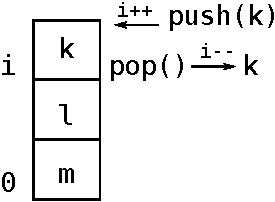
\includegraphics[scale=0.50]{fig/stack.pdf}
\end{center}
\end{wrapfigure}

\Question \label{ex:stack q2} Bonus. Write a \func{String} method which 
converts the stack to a string. This way you can print the stack using:
\lstinline{fmt.Printf("My stack %v\n", stack)}. This may aid in
debugging.
\end{Exercise}

\begin{Answer}

\Question 

\Question 

\end{Answer}


\begin{Exercise}[title={Stack as package},difficulty=2]
\label{ex:stack-package}
\Question\label{ex:stack-package q1} Create a proper package for your
stack implementation, \func{push}, \func{pop} and the \type{stack} type need to be
exported.

\Question\label{ex:stack-package q2} Which official Go package could
also be used for a (FIFO) stack?

\end{Exercise}

\begin{Answer}
\Question There are a few details that should be changed to make a proper package
for our stack. First, the exported function should begin with a capital 
letter and so should \type{Stack}. So the full package (including the
\func{String()} function becomes
\lstinputlisting[caption=Stack in a
package]{ex-functions/src/stack-as-package.go}

\Question The \package{container/vector} package would be a could candidate. It
even comes with \func{push} and \func{pop} functions \emph{predefined}.
\end{Answer}


\begin{Exercise}[title={Calculator},difficulty=7]
\label{ex:cacl}
\Question\label{ex:calc q1} Create a reverse polish calculator, use your
stack package.

\end{Exercise}

\begin{Answer}
\end{Answer}


\cleardoublepage
\section{Answers}
\shipoutAnswer
